\documentclass[11pt,letterpaper]{article}

% \usepackage{epstopdf}% To incorporate .eps illustrations using PDFLaTeX, etc.
% \usepackage[caption=false]{subfig}% Support for small, `sub' figures and tables
%\usepackage[nolists,tablesfirst]{endfloat}% To `separate' figures and tables from text if required
%\usepackage[doublespacing]{setspace}% To produce a `double spaced' document if required
%\setlength\parindent{24pt}% To increase paragraph indentation when line spacing is doubled

% \usepackage[longnamesfirst,sort]{natbib}% Citation support using natbib.sty
% \bibpunct[, ]{(}{)}{;}{a}{,}{,}% Citation support using natbib.sty
% \renewcommand\bibfont{\fontsize{10}{12}\selectfont}% To set the list of references in 10 point font using natbib.sty

\usepackage[natbibapa,nodoi]{apacite}% Citation support using apacite.sty. Commands using natbib.sty MUST be deactivated first!
\setlength\bibhang{12pt}% To set the indentation in the list of references using apacite.sty. Commands using natbib.sty MUST be deactivated first!
\renewcommand\bibliographytypesize{\fontsize{10}{12}\selectfont}% To set the list of references in 10 point font using apacite.sty. Commands using natbib.sty MUST be deactivated first!
\usepackage[english]{babel}
\addto{\captionsenglish}{%
    \renewcommand{\refname}{Referanslar}%
    \renewcommand{\contentsname}{Table of Contents}}

% \theoremstyle{plain}% Theorem-like structures provided by amsthm.sty
% \newtheorem{theorem}{Theorem}[section]
% \newtheorem{lemma}[theorem]{Lemma}
% \newtheorem{corollary}[theorem]{Corollary}
% \newtheorem{proposition}[theorem]{Proposition}

% \theoremstyle{definition}
% \newtheorem{definition}[theorem]{Definition}
% \newtheorem{example}[theorem]{Example}

% \theoremstyle{remark}
% \newtheorem{remark}{Remark}
% \newtheorem{notation}{Notation}

\usepackage[table,x11names,svgnames,dvipsnames]{xcolor}
\usepackage[export]{adjustbox}
% \usepackage{algorithm}
% \usepackage[noend]{algpseudocode}
\usepackage{amsmath,amssymb,amsfonts}
\usepackage[USenglish]{babel}
\usepackage{bigints}
\usepackage{bm}
\usepackage{booktabs}
\usepackage{cancel}
\usepackage[tableposition=above, font=normalsize]{caption}
% \usepackage{centernot}
% \usepackage{comment}
\usepackage{empheq}
\newcommand*\widefbox[1]{\fbox{\hspace{2em}#1\hspace{2em}}}
\usepackage{enumitem}
\usepackage{epsfig}
\usepackage{epstopdf}
% \epstopdfsetup{outdir=./figures//}
% \usepackage[letterpaper, top=1.0in, bottom=1.0in, left=1.0in, right=1.0in]{geometry}
\RequirePackage[OT1]{fontenc}
% \usepackage{fontspec}
\usepackage{graphics}
\usepackage{graphicx}
\graphicspath{{../figures/}}
% \usepackage{ifpdf}
% \usepackage{lastpage}
% \usepackage{leftidx}
\usepackage{lineno}
\usepackage{lipsum}
% \usepackage{mathrsfs}
\usepackage{mathtools}
\usepackage{multicol}
\usepackage{multirow}
\usepackage{nicefrac}
% \usepackage{nicematrix}
% \usepackage{pgfplots}
\usepackage{pifont}
% \usepackage{ragged2e}
% \usepackage{rotating}
% \usepackage{stmaryrd}
\usepackage{siunitx}
\usepackage{soul}
\usepackage[caption=false]{subfig}
\usepackage{tabularx}
\usepackage{threeparttable}
\usepackage{tikz}
% \usepackage{tkz-euclide}
% \usepackage{ctable}
% \usetikzlibrary{matrix, arrows}
\usetikzlibrary{shapes.geometric, arrows, decorations.markings, shapes.arrows}

\newcommand{\minitab}[2][l]{\begin{tabular}{#1}#2\end{tabular}}

%%%%%%% TODO NOTES 
\usepackage{todonotes}
\setlength{\marginparwidth}{1.3cm}
\setlength{\marginparsep}{0cm}
\newcommand{\ctodo}[1]{\todo[size=\tiny]{#1}}
\newcommand{\nnparam}{\theta}
\newcommand{\pinn}{\pi_{\nnparams}}

\usepackage{wrapfig}

\tikzstyle{startstop} = [rectangle, rounded corners, minimum width=1cm, minimum
height = 0.5cm, text centered, draw=black, fill=red!30]
\tikzstyle{io} = [trapezium, trapezium left angle=70, trapezium right angle=110,
minimum height=1cm, text width=3cm, text centered, draw=black, fill=blue!30]
\tikzstyle{process} = [rectangle, minimum width=2cm, minimum height=0.8cm, text
centered, text width=2cm, draw=black, fill=orange!30]
\tikzstyle{decision} = [diamond, aspect=1.25, minimum width=2cm, minimum height=0.5cm, 
text centered, text width=3cm, draw=black, fill=green!30]
\tikzstyle{arrow} = [thick, ->, >=stealth]




\makeatletter
\newcommand{\rmnum}[1]{\romannumeral #1}
\newcommand{\Rmnum}[1]{\expandafter\@slowromancap\romannumeral #1@}
\makeatother

\newcommand{\bmat}[1]{\begin{bmatrix}#1\end{bmatrix}}
\newcommand{\pmat}[1]{\begin{pmatrix}#1\end{pmatrix}}
\newcommand{\ubar}[1]{\text{\b{$#1$}}}
\newcommand{\norm}[2]{\|{#1}\|_{{}_{#2}}}
\newcommand{\abs}[1]{\left|{#1}\right|}
\newcommand{\mbf}[1]{\mathbf{#1}}
\newcommand{\mc}[1]{\mathcal{#1}}
\newcommand{\dd}{\operatorname{d}\!}
\newcommand{\muc}[2]{\multicolumn{#1}{c}{#2}}
\newcommand*\Eval[3]{\left.#1\right\rvert_{#2}^{#3}}
\newcommand{\inner}[1]{\left\langle#1\right\rangle}
\newcommand{\pd}[2]{\frac{\partial #1}{\partial #2}}
\newcommand{\pdd}[2]{\frac{\partial^2 #1}{\partial #2^2}}
\newcommand{\el}[2]{\frac{\dd}{\dd t}\pd{\mc{L}}{\dot{#1}} - \pd{\mc{L}}{#1} = #2}
\newcommand{\elk}[2]{\frac{\dd}{\dd t}\pd{\mc{L}}{\dot{#1}_k} - \pd{\mc{L}}{#1_k} = #2_k}
\newcommand{\vectornorm}[1]{\left|\left|#1\right|\right|}
\newcommand{\dom}[1]{\textrm{dom}\;#1}
\newcommand{\bx}{{\bf x}}
\newcommand{\bu}{{\bf u}}
\newcommand{\cmark}{\ding{51}}%
\newcommand{\xmark}{\ding{55}}%
\newcommand*{\vertbar}{\rule[-1ex]{0.5pt}{2.5ex}}
\newcommand*{\horzbar}{\rule[.5ex]{2.5ex}{0.5pt}}

\newcommand{\idapbc}{\textsc{IdaPbc}}
\newcommand{\electric}{{\textcolor{blue}{\hspace{-0.5mm}$\bm{E}$\;}}}
\newcommand{\magnetic}{{\textcolor{red}{\hspace{-0.5mm}$\bm{B}$\;}}}

% \theoremstyle{plain}
% \newtheorem{thm}{Theorem}[section]
\newtheorem{thm}{Theorem}
% \makeatletter
% \@addtoreset{thm}{section}
% \makeatother
% \newtheorem{cor}[thm]{Corollary}
\newtheorem{lem}{Lemma}
% \newtheorem{claim}[thm]{Claim}
% \newtheorem{axiom}[thm]{Axiom}
% \newtheorem{conj}[thm]{Conjecture}
% \newtheorem{fact}[thm]{Fact}
% \newtheorem{hypo}[thm]{Hypothesis}
% \newtheorem{assum}[thm]{Assumption}
\newtheorem{prop}{Proposition}
% \newtheorem{crit}[thm]{Criterion}
% \theoremstyle{definition}
\newtheorem{defn}[thm]{Definition}
% \newtheorem{exmp}[thm]{Example}
\newtheorem{rem}{Remark}
% \newtheorem{prin}[thm]{Principle}

\DeclareMathOperator{\Tr}{tr}
\newcommand\xdownarrow[1][2ex]{%
   \mathrel{\rotatebox{90}{$\xleftarrow{\rule{#1}{0pt}}$}}
}
\DeclareMathOperator{\End}{End}
\DeclareMathOperator{\Hom}{Hom}
\DeclareMathOperator{\id}{id}
\DeclareMathOperator{\vers}{vers}
\DeclareMathOperator{\trans}{Trans}
\DeclareMathOperator{\rot}{Rot}
\DeclareMathOperator{\rank}{rank}
\DeclareMathOperator{\sinc}{sinc}

\usepackage{hyperref}
\hypersetup{
    unicode=false,          % non-Latin characters in Acrobat’s bookmarks
    pdftoolbar=true,        % show Acrobat’s toolbar?
    pdfmenubar=true,        % show Acrobat’s menu?
    pdffitwindow=false,     % window fit to page when opened
    pdfstartview={FitH},    % fits the width of the page to the window
    pdftitle={Mischievous Sibling's Grid World},    % title
    pdfauthor={Aykut C. Satici}, % author
    % pdfsubject={Subject},   % subject of the document
    % pdfcreator={Creator},   % creator of the document
    % pdfproducer={Producer}, % producer of the document
    % pdfkeywords={keyword1, key2, key3}, % list of keywords
    pdfnewwindow=true,      % links in new PDF window
    colorlinks=true,       % false: boxed links; true: colored links
    linkcolor=blue!30!green,          % color of internal links (change box color with linkbordercolor)
    linkbordercolor=orange,
    citecolor=blue,        % color of links to bibliography
    citebordercolor=green,
    filecolor=magenta,      % color of file links
    urlcolor=cyan,           % color of external links
    urlbordercolor=blue,
}


\begin{document}

% \articletype{}% Specify the article type or omit as appropriate

% \title{\.{I}lgin\c{c} Bir Olas{\i}l{\i}k Sorusu}
\section*{
    \begin{center}
        \.{I}lgin\c{c} Bir Olas{\i}l{\i}k Sorusu
    \end{center}
}

\begin{center}
    G\"{o}khan At{\i}n\c{c}\textsuperscript{} ve Aykut C. Sat{\i}c{\i}\textsuperscript{} \\[0ex]
    % 1 Temmuz 2021
\end{center}

% \author{
% \name{G\"{o}khan At{\i}n\c{c}\textsuperscript{\dagger} and Aykut C. Sat{\i}c{\i}\textsuperscript{\ddagger}}
% \affil{\textsuperscript{\dagger}Boise State University, Electrical and Computer Enginering Department, Boise, Idaho, USA}
% }

% \maketitle


% \begin{abstract}
%   Machine learning approaches to the problem of control design are flexible,
%   but they demand large databases and computation time for training. Part of
%   this central challenge is due to treating the environment as a black box,
%   ignoring the useful geometric or algebraic structures of the control system.
%   In this work, we propose an efficient data-driven procedure that leverages
%   the known dynamics and techniques from nonlinear control theory in order to
%   design swing-up controllers for underactuated robotic systems. We embed a
%   neural network into the equations of motion of the robotic manipulator
%   through its control input. This control function is determined by the
%   appropriate gradients of a neural network, acting as an energy-like
%   (Lyapunov) function. We encode the swing-up task through the use of
%   transverse coordinates and goal sets; which provides a concise target for
%   the neural network and drastically accelerates the rate of learning. We
%   demonstrate the efficacy and robustness of the algorithm with numerical
%   simulations and experiments on hardware.
% \end{abstract}
  
% \begin{keywords}
%   Sections; lists; figures; tables; mathematics; fonts; references; appendices
% \end{keywords}

  
\vspace{-1mm}
\section{Problem Statement}

\definecolor{blue538}{HTML}{30a2da}
\definecolor{red538}{HTML}{fc4f30}
\definecolor{yellow538}{HTML}{e5ae38}
\definecolor{green538}{HTML}{6d904f}
\definecolor{gray538}{HTML}{8b8b8b}
%
% \begin{wrapfigure}{r}{0.4\textwidth} %this figure will be at the right
%     \vspace{-5mm}
%     \centering
%     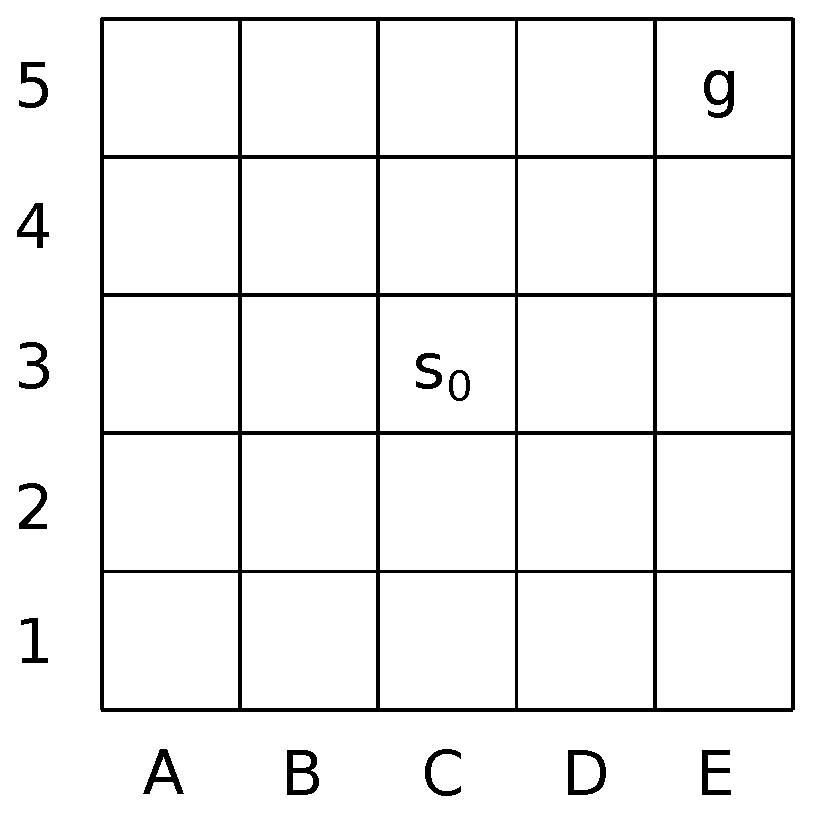
\includegraphics[width=0.25\textwidth]{./figures/drawing.eps}
%     \caption{Problemin \c{s}emati\u{g}i}
%     \label{fig:schematic}
%     \vspace{-5mm}
% \end{wrapfigure}
%
\begin{minipage}{0.5\textwidth}
    Points $P$ and $Q$ are randomly sampled from a uniform distribution on two
    sides of a unit square. Let $d$ be the random variable that denotes the
    length of the chord $\abs{PQ}$ (see the figure). What is the probability
    that $d \geq 1$?
\end{minipage}
\begin{minipage}{0.5\textwidth}
    \begin{center}
\begin{tikzpicture}[scale=2]
    % \draw (0, 0) -- (1.5, 0);
    % \draw (0, 0) -- (0, 1.5);
    %
    % \draw[ultra thin, gray, step=.1cm] (0, 0) grid (1.5, 1.5);
    %
    % \draw[ultra thick, blue538] (0, 0) rectangle (1, 1);
    \draw[ultra thick] (0, 0) rectangle (1, 1);
    %
    \foreach \x/\xtext in {0, 1}
    \draw (\x cm, 1pt) -- (\x cm,-1pt) node[anchor=north] {$\xtext$};
    \foreach \y/\ytext in {0, 1}
    \draw (1pt,\y cm) -- (-1pt,\y cm) node[anchor=east] {$\ytext$};
    %
    \node[above] (P) at (0.6, 1) {$P$};
    \node[right] (Q) at (1, 0.2) {$Q$};
    \draw (0.6, 1) -- (1, 0.2);
    \draw[fill=black] (0.6, 1) circle (.03cm);
    \draw[fill=black] (1, 0.2) circle (.03cm);
\end{tikzpicture}
\end{center}
\end{minipage}

\section{Problem Solution}
\label{sec:solution}

Shown in Figure~\ref{fig:unfolded}, we show the regular pyramid of
Figure~\ref{fig:problem} unfolded onto the plane in such a manner that the edge
$OQ$ remains glued, while the edges $OR$, $OS$, and $OP$ are unglued. An
arbitrary piecewise straight path $\gamma$ from the vertex $P$ to the midpoint
$T$ is then depicted as the green curve on this figure. The continuous portions,
$PU$ and $UT$, of this path have lengths $\ell_1$ and $\ell_2$, respectively.

The line $PR$ that connects the vertices $P$ and $R$ is orthogonal to the edge
$OQ$ since the triangle $\triangle POQ$ is equilateral. Let the signed distance
from the intersection $M$ of $PR$ with $OQ$ to the intersection $U$ of our path
$\gamma$ and $OQ$ be given by $x$. In the following, we express the total length
$\ell_1 + \ell_2$ of our curve $\gamma$ as a function of this distance $x$ and
minimize it to arrive at the answer.

\begin{figure}[h]
  \centering
  \includegraphics[trim={0 0 0
  0cm},clip,width=0.5\textwidth]{./figures/pyramid-unfolded.pdf}
  \vspace{-8mm}
  \caption{The unfolded regular pyramid.}
  \label{fig:unfolded}
\end{figure}

Since $PM \perp OM$, Pythagoras's theorem yields $\abs{PM} = \sqrt{3}\ell$. By
the same token, $\triangle PMU$ is a right triangle, yielding 
%
\begin{equation}
    \ell_1(x) = \sqrt{x^2 + 3\ell^2}. 
    \label{eq:ell1}
\end{equation}    
%
The perpendicular $TM^\prime$ to $PR$ is parallel to $OQ$ so by the similarity
of the triangles $\triangle OMR$ and $\triangle TM^\prime R$, and the fact that
$\abs{OM} = \ell$, we deduce that $\abs{TM^\prime} = \nicefrac{\ell}{2}$ and
$\abs{MM^\prime} = \nicefrac{\sqrt{3}\ell}{2}$. Using these lengths, along with
$x$, as the side lenghts of the orange right triangle $\triangle T\tilde{M}M$ in
Figure~\ref{fig:unfolded}, we obtain 
%
\begin{equation}
  \ell_2(x) = \sqrt{\ell^2 + \ell x + x^2}.
  \label{eq:ell2}
\end{equation}

The solution that we seek minimizes $\ell_1(x) + \ell_2(x)$. Therefore, we
differentiate this function and set it equal to zero to obtain \[
\frac{2x}{\sqrt{3\ell^2 + x^2}} + \frac{\ell+2x}{\sqrt{\ell^2 + \ell x + x^2}} =
0. \] The solution to this equation is $x^\star = -\nicefrac{\ell}{3}$ as a
simple substitution will show. Plugging this solution into
equations~\eqref{eq:ell1} and~\eqref{eq:ell2} yields \[ \ell_1^\star =
\ell_1(x^\star) = \frac{2\sqrt{7}}{3}\ell, \qquad \ell_2^\star =
\ell_2(x^\star)= \frac{\sqrt{7}}{3}\ell. \] Summing these two optimal values
gives the shortest distance between points $P$ and $T$ on the regular square
pyramid as \[ \ell_1(x^\star) + \ell_2(x^\star) = \sqrt{7}\ell. \]

\begin{lemma}{\textbf{Lemma 1.}}
  The (green) path that yields the shortest distance $\sqrt{7}\ell$ is a
  straight line.
\end{lemma}

\begin{proof}
    Perhaps the easiest way to show this is to use the law of cosines to show
    that the edge $PT$ of the triangle $\triangle POT$ has length equal to
    $\sqrt{7}\ell$ so that our solution for the green path coincides with the
    dash-dotted red line on Figure~\ref{fig:unfolded}.

    \begin{align*}
        \abs{PT}_{\text{red}}^2 &= (2\ell)^2 + \ell^2 - 2 \cdot 2\ell \cdot \ell
        \cos{120^\circ} = 7\ell^2
    \end{align}
\end{proof}

% \section{Methods}
\label{sec:methods}

The goal of this paper to systematically design a stabilizing controller using a
learning-based framework. To this end, we carefully combine the universal function
approximation capability of neural networks with the intrinsic stabilization
properties of passivity-based control theory. In particular, we tackle the task
of solving the matching PDEs~\eqref{eq:pde_main} by formulating a neural network
optimization problem and imposing the relevant constraints, which are elaborated in
the subsequent subsections.

%%%%%%%%%%%%%%%%%%%%%%%%%%%%%%%%%%%%%%%%%%%%%%%%%%%%%%%%%%%%%%%%%%%

\subsection{Main Learning Problem}
\label{ssec:pinn}


The IDA-PBC design can be formulated as the following feasibility problem:
%
% \begin{equation}
%     \begin{aligned}
%         \underset{M_d,\, J_2,\, V_d }{\textrm{minimize}} 
%         &&\quad J &= \int_{\mathcal{X}} \; \Bigl\| \, l(x) \, \Bigr\|^2 \; \dd x, \\
%         \textrm{subject to} 
%         &&\quad M_d &= M_d^\top \succ 0, \\
%         &&\quad J_2 &= -J_2^\top, \\
%         &&\quad q^\star &= \underset{q}{\textrm{argmin}} \; V_d.  \\
%     \end{aligned}    
%     \label{eq:infinite_optim}
% \end{equation}
\begin{equation}
    \begin{aligned}
        \underset{M_d,\, J_2,\, V_d }{\textrm{minimize}} && 0 &, \\
        \textrm{subject to} 
        &&\quad 0 &= G^\perp \left( \nabla_qH - M_dM^{-1} \nabla_qH_d + J_2M_d^{-1}p \right), \\
        &&\quad H_d &= \textrm{Eq.~\eqref{eq:desired_hamiltonian}}, \\
        &&\quad M_d &= M_d^\top \succ 0, \\
        &&\quad J_2 &= -J_2^\top, \\
        &&\quad q^\star &= \underset{q}{\textrm{argmin}} \; V_d.  \\
    \end{aligned}    
    \label{eq:infinite_optim}
\end{equation}
%
This is an infinite-dimensional, nonlinear optimization problem that is
intractable to solve in closed-form. We therefore seek to reduce the problem to
a finite-dimensional one through the means of approximation by neural networks.

To this end, we proceed by representing the candidate solutions $M_d(q)$ and
$J_2(q,p)$ by fully-connected neural networks $M_d^{\theta_m}: \mathbb{R}^n \to
\mathbb{R}^{n \times n}$ and $J_2^{\theta_j}: \mathbb{R}^{2n} \to \mathbb{R}^{2n
\times 2n}$, where $\theta_m \in \mathbb{R}^{n_m}$ and $\theta_j \in
\mathbb{R}^{n_j}$ each denote the corresponding neural network parameters. 
%
% To accommodate the isolated minimum requirement of $V_d(q)$, we opt to
% approximate it with a Sum-of-Squares (SoS) polynomial, denoted by
% $V_d^{\theta_v}: \mathbb{R}^{n} \to \mathbb{R}$, with $\theta_{n_v}$
% representing the polynomial coefficients. 
%
We opt to approximate $V_d(q)$ with a Sum-of-Squares (SoS) polynomial of degree $2d$, denoted
by $V_d^{\theta_v}: \mathbb{R}^{n} \to \mathbb{R}$, with $\theta_{n_v} \in \mathbb{R}^{n_v}$
representing the polynomial coefficients. 
%
For compactness, we shall refer to these function approximators as
$M_d^\theta, J_2^\theta, V_d^\theta$ henceforth.

\begin{definition}[SoS Polynomial] \label{def:sos_poly}
    A polynomial $P \in \mathbb{R}[x]$ of degree $d = \eta_1 + \cdots +
    \eta_n$, $\eta_i \in \mathbb{N}$, i.e.,
    %
    \begin{equation*}
      P(x) = \sum_{\eta_1 + \cdots + \eta_n \leq d} c_\eta x_1^{\eta_1}
             \cdots x_n^{\eta_n}
    \end{equation*}
    %
    is a sum-of-squares if there exist a finite number of polynomials
    $P_i \in \mathbb{R}[x]$ such that $P$ can be written as
    %
    $%\begin{equation*}
      P(x) = \sum_i P_i^2(x).
    $%\end{equation*}
\end{definition}

\begin{remark}
    Note that if $P(x)$ is SoS, then $P(x) \geq 0\ \forall x \in \mathbb{R}^n$.
    If the constant term is zero, i.e. $c_0 = 0$, then $P(x) = 0 \iff x = 0$.
    Without loss of generality, this suggests a natural way to impose the
    isolated minimum requirement of $V_d(q)$ by shifting the coordinate of $q$
    and aligning $q^\star$ with the origin. Further, SoS polynomials can be
    parametrized by the (convex) set of positive semidefinite matrices. This
    simplifies the search for a SoS polynomial $V_d^{\theta}$ that best
    satisfies~\eqref{eq:pde_2} once $M_d^{\theta}, J_2^\theta$ are identified.
\end{remark}

Let $\theta := (\theta_m, \theta_j, \theta_v) \in \mathbb{R}^{n_\theta}$ with
$n_\theta = n_m + n_j + n_v$.
%
With $x = (q, p)$, define the loss function $l_\theta(x)$ as the
inner product of the left-hand-side (LHS) of Eq.~\eqref{eq:pde_main}, i.e.
%
\begin{equation}
    l_\theta(x) = \left\| G^\perp \left( \nabla_qH - M_d^\theta M^{-1} \nabla_q H_d^\theta + J_2^\theta {M_d^\theta}^{-1}p \right) \right\|^2,
    \label{eq:loss_nn}
\end{equation}
%
where $H_d^\theta(q,p) = \frac{1}{2} p^\top \left(M_d^\theta\right)^{-1} p +
V_d^\theta(q)$.
%
The proposed framework aims to approximate the solution
to~\eqref{eq:infinite_optim} by finding the parameters $\theta$ such that
$l_\theta$ is minimized over the appropriate region $\Omega$ of the state space,
i.e. $\Omega \subset \mathcal{X}$. We arrive at the following finite-dimensional
optimization problem:
%
\begin{equation}
    \begin{aligned}
        \underset{\theta }{\textrm{minimize}} 
        &&\quad J &= \sum_{x \in \Omega} l_\theta (x) , \\
        \textrm{subject to} 
        &&\quad M_d^\theta &= \big( M_d^\theta \big)^\top \succ 0, \\
        &&\quad J_2^\theta &= -\big( J_2^\theta \big)^\top, \\
        % &&\quad q^\star &= \underset{q}{\textrm{argmin}} \; V_d^\theta.  \\
        &&\quad V_d^\theta (q) &\textrm{ is SoS}, \\
        &&\quad V_d^\theta (q^\star) &= 0.
    \end{aligned}    
    \label{eq:finite_optim}
\end{equation}

\todo[inline]{Insert connection to Physics-Informed neural networks (PINN) here.} 
As $J \rightarrow 0$, the function approximators $M_d^\theta, J_2^\theta,
V_d^\theta$ converge to the solutions of the PDE~\eqref{eq:pde_main} governing
the stabilization properties of IDA-PBC.


%%%%%%%%%%%%%%%%%%%%%%%%%%%%%%%%%%%%%%%%%%%%%%%%%%%%%%%%%%%%%%%%%%%

\subsection{Constraints}
\label{ssec:pinn}

In the subsequent subsections, we elaborate on how the constraints
in the optimization problem~\eqref{eq:finite_optim} are imposed. 
%
For the remainder of this document, we shall let $\mathbb{S}_n$ denote the set
of symmetric $n \times n$ matrices, $\mathbb{S}^{+}_n$ the set of positive
semidefinite $n \times n$ matrix, and $\mathbb{S}^{++}_n$ the set of positive
definite $n \times n$ matrix.

\subsubsection{Positive-Definiteness of $M_d^\theta$ and Skew-Symmetry of $J_2^\theta$}

We leverage the Cholesky decomposition to ensure positive-definiteness of
$M_d^\theta$, i.e.,
%
\begin{equation}
    M_d^\theta(q) = L_{\theta}(q) L_{\theta}^\top(q),
    \label{eq:cholesky}
\end{equation}
%
where $L_\theta \in \mathbb{R}^{n \times n}$ is a lower-triangular matrix whose
$n(n+1)/2$ entries are outputs of a neural network. The positive-definiteness is
ensured as long as the diagonal elements of $M_d^\theta$ are positive. In our
implementation, this is achieved by adding $\epsilon I$ to $M_d^\theta$, with
$I$ denoting the identity matrix and $\epsilon$ a small positive constant.

The skew symmetric $J_2^\theta$ is constructed by taking a square matrix
$A_\theta$, whose entries are outputs of a dense neural network, and compute
%
\begin{equation}
    J_2^\theta(q,p) = A_\theta(q,p) - A_\theta^\top (q,p).
    \label{eq:skew_symmetric}
\end{equation}

\subsubsection{Positivity of $V_d^\theta$ with An Isolated Minimum at $q^\star$}

By Definition~\ref{def:sos_poly}, a polynomial function is nonnegative as long
as it is SoS. We therefore are concerned with constructing the polynomial
$V_d^\theta$ as an SoS polynomial. 
%
\begin{theorem}~\citep{choi1995sums}
    \label{thm:sos}
    A polynomial $P \in \mathbb{R}[x]$ of degree $2d$ has a sum-of-squares
    decomposition if and only if there exists a $Q \in \mathbb{S}^{+}_n$ such
    that
    %
    \begin{equation*}
        P(x) = m^\top(x) Q m(x),
    \end{equation*}
    %
    where $m$ is the vector of all monomials in $x_1, \ldots, x_n$ of
    degree less than or equal to $d$, i.e. $m(x) = \bmat{1 & x_1 & x_2 & \ldots &
    x_n & x_1x_2 & \ldots & x_n^d}$. There exist $\binom{n+d}{n}$ such monomials.
\end{theorem}

This result presents an efficient way to construct $V_d^\theta$. The SoS
constraint in~\eqref{eq:finite_optim} is then equivalent to finding a positive
semidefinite matrix. We use the same Cholesky decomposition
in~\eqref{eq:cholesky} to do this. With $R_\theta$ an $n \times n$ lower
triangular matrix with constant entries, we define 
%
\begin{equation}
    V_d^\theta(q) = m^\top(q) R_\theta R_\theta^\top m(q),
    \label{eq:sos_Vd}
\end{equation}
%
where $m$ is the vector of monomials $m = \bmat{q_1 & \ldots & q_n &
q_1q_2 & \ldots & q_n^d}$. The constant monomial is excluded from $m(q)$ to
ensure that the minimum of $V_d^\theta$ is at the origin.


%%%%%%%%%%%%%%%%%%%%%%%%%%%%%%%%%%%%%%%%%%%%%%%%%%%%%%%%%%%%%%%%%%%

\subsection{Reducing the Sample Space}
\label{ssec:sample}

% We are interested in finding the solution to~\eqref{eq:finite_optim} over the
% region $\Omega \subset \mathcal{X}$. 
%
In this subsection, we show how the loss function~\eqref{eq:loss_nn} can be
expressed in a more explicit form which only depends on the variable $q$ instead
of $(q,p)$. This reduces the sample complexity of the algorithm by half. 
Following~\cite{ortega2002stabilization}, we use the fact that
%
\[
    \nabla_q \left(z^\top A(q) z \right) = 
    \left[ \nabla_q \left( A(q)z \right)\right]^\top z,
    \; \forall z \in \mathbb{R}^n, \; \forall A \in \mathbb{S}_n,
\]
%
to write the PDE constraint~\eqref{eq:pde_1} as
%
\begin{equation*}
    G^\perp \left\{ \left[
        \left[ \nabla_q \left( M^{-1} p \right) \right]^\top - 
        M_d M^{-1} \left[ \nabla_q \left( M_d^{-1} p \right) \right]^\top + 
        2 J_2 M_d^{-1} 
    \right] p \right\}= 0.
\end{equation*}
%
The identity
%
$
    \nabla_q \left( A(q) z \right) = \sum_{k=1}^n \nabla_q \left( A_{(\cdot, k)} \right) z_k,
$
%
where $A_{(\cdot, k)}$ denotes the $k^\textrm{th}$ column of the matrix $A$,
holds for all $z \in \mathbb{R}^n$ and all $A \in \mathbb{R}^{n \times n}$. We
use this identity to reparametrize $J_2^\theta$ in terms of the matrices $U_k^\theta(q) =
\left(-U_k^\theta (q)\right)^\top \in \mathbb{R}^{n \times n}$ as
%
\[
    2 J_2^\theta = \sum_{k=1}^n U^\theta_k p_k.
\]

We can now express~\eqref{eq:loss_nn} only in terms of $q$ as $l_\theta =
\left( \sum_{k=1}^n l_{1k,\theta} \right) + l_{2,\theta}$, where
% %
% \begin{equation}
%     G^\perp \left\{ 
%         \left[ \nabla_q \left( M^{-1}_{(\cdot, k)} \right) \right]^\top - 
%         M_d M^{-1} \left[ \nabla_q  \left( M_d^{-1}\right)_{(\cdot, k)} \right]^\top + 
%         U_k M_d^{-1} 
%     \right\}= 0.
%     \label{eq:pde_1_revised}
% \end{equation}
% %
% These results elude us to decompose~\eqref{eq:finite_optim} into two smaller
% optimization problems. First we express the loss functions~\eqref{eq:loss_nn}
% into two terms as
% %
\begin{align}
    \label{eq:loss_decoupled_1}
    l_{1k, \theta}(q) &= \left\| G^\perp \left\{ 
        \left[ \nabla_q \left( M^{-1}_{(\cdot, k)} \right) \right]^\top - 
        M_d^{\theta} M^{-1} \left[ \nabla_q  \left( \big( M_d^\theta \big)^{-1} \right)_{(\cdot, k)} \right]^\top + 
        U_k^\theta \big( M_d^\theta \big)^{-1}
    \right\} \right\|^2 , \\
    \label{eq:loss_decoupled_2}
    l_{2, \theta}(q) &= \left\| G^\perp \left\{ \nabla_qV - M_d^\theta M^{-1} \nabla_qV_d^\theta \right\} \right\|^2.
\end{align}
%
Note that~\eqref{eq:loss_decoupled_1} is only dependent of $M_d^\theta$ and
$U_k^\theta$. This implies that the problem~\eqref{eq:finite_optim} can be
solved in two stages, as elaborated in the following subsection.


\subsection{Solving the Optimization Problem}

We rewrite the problem~\eqref{eq:finite_optim} into two smaller problems, first
of which is
%
\begin{equation}
    \begin{aligned}
        \underset{\theta }{\textrm{minimize}} 
        &&\quad J_1 &= \sum_{q \in \mathcal{Q}} \left( \sum_{k=1}^n l_{1k,\theta}(q) \right) , \\
        \textrm{subject to} 
        &&\quad M_d^\theta &= \big( M_d^\theta \big)^\top \succ 0, \\
        &&\quad U_k^\theta &= -\big( U_k^\theta \big)^\top, \;\; k = 1,\ldots,n.
    \end{aligned}    
    \label{eq:solve_Md}
\end{equation}
%
To solve this optimization problem, we exploit the recent developments in
automatic differentiation (AD)~\citep{DifferentialEquations.jl-2017} to obtain
the appropriate gradients for use with gradient-based search algorithms. In
particular, we employ the reverse-mode AD implemented in the Julia language
(\verb|ReverseDiff.jl|) and perform parameter updates according to
ADAM~\citep{kingma2014adam}.

Given the solutions $M_d^\theta, U_k^\theta$ to~\eqref{eq:solve_Md}, the
following optimization problem can be solved to obtain the coefficients of
$V_d^\theta$:
%
\begin{equation}
    \begin{aligned}
        \underset{\theta }{\textrm{minimize}} 
        &&\quad J_2 &= \sum_{q \in \mathcal{Q}} l_{2,\theta}(q), \\
        \textrm{subject to} 
        &&\quad V_d^\theta (q) &\textrm{ is SoS}, \\
        &&\quad V_d^\theta (q^\star) &= 0.
    \end{aligned}    
    \label{eq:solve_Vd}
\end{equation}
%
As the gradient of~\eqref{eq:sos_Vd} can be analytically obtained, the
problem~\eqref{eq:solve_Vd} can be re-formulated as the least squares problem:
$\min\|Ax - b\|^2$. This problem is then solved in a single step, significantly
increasing the computation speed of our algorithm.
% 

\subsection{Case Study I: Inertia-Wheel Pendulum}
\label{sec:iwp}

In this section, we apply the design methodology to the problem of stabilizing
the inverted position of an inertia wheel pendulum (IWP), shown in
Fig.~\ref{fig:iwp}. 

This mechanism is a simple pendulum with an actuated wheel instead of a static
bob.
%
The wheel has mass $m$, which is connected to a massless rod of length \(l\). 
%
The rod is connected to ground by a revolute joint, whose position
is denoted by the angle \(\theta_1\) measured with respect to the downward
vertical position.
%
The position of the wheel \(\theta_2\) is measured with respect to the vertical
line through the center of the wheel.

\begin{figure}[tb]
    \centering
    \includegraphics[width=0.27\linewidth]{figures/iwp.eps}
    \caption{Schematic of the inertia wheel pendulum. The rotating wheel \(\theta_2\) is actuated.}
    \label{fig:iwp}
\end{figure}

\subsubsection{System Model}

The Hamiltonian is $H = \frac{1}{2} p^\top M^{-1} p + V(q)$, with $p = \bmat{I_1
\dot{q}_1 & I_2 \dot{q}_2}^\top$ and
%
\begin{equation*}
    M = \bmat{I_1 & 0 \\ 0 & I_2},
    \quad
    G = \bmat{-1 \\ \phantom{-}1},
    \quad
    V(q) = mgl \left( \cos q_1 - 1 \right).
\end{equation*}
%
Here \(I_1\) denotes the moment of inertia of the pendulum, \(I_2\) is the moment of
inertia of the rotating wheel, \(g\) is the gravitational constant, and $l$ is
the length of the rod. The equilibrium to be stabilized is the upward position $(q_1^\star, q_2^\star) = (0, 0)$.
%
The equations of motion of the IWP can be written in standard form as 
%
\begin{equation*}
    % \begin{aligned}
    %     I_1\ddot{\theta}_1 &= -mgl \sin(\theta_1) - u, \\
    %     I_2\ddot{\theta}_2 &= u
    % \end{aligned}
    \bmat{I_1 & 0 \\ 0 & I_2} \bmat{q_1 \\ q_2} + \bmat{-mgl \sin q_1 \\ 0} = \bmat{-1 \\ \phantom{-}1} u, 
\end{equation*}
%
where the control input \(u\) is the torque applied to the inertia wheel.
%
The following values are used for system parameters: \(I_1
= 0.1,\, I_2 = 0.2\), and $mgl = 10$. 


\begin{table}[b]
    \caption{Neural network architectures for solving~\eqref{eq:solve_Md} in the IWP case study. The ordering of the layer dimensions and activations are arranged from input to output. }
    \centering
    \begin{tabular}{r|c|c}
         & Layer Dimensions  & Activation Functions \\ \hline
        $M_d^\theta$ Equation~\eqref{eq:cholesky} & (2, 16, 16, 3) & (ELU, ELU, ELU, Identity) \\
        $U_1^\theta$ Equation~\eqref{eq:skew_symmetric} & (2, 8, 8, 1) & (ELU, ELU, ELU, Identity) \\
        $U_2^\theta$ Equation~\eqref{eq:skew_symmetric} & (2, 8, 8, 1) & (ELU, ELU, ELU, Identity) \\ 
    \end{tabular}
    \label{tab:iwp_nn}
\end{table}

\subsubsection{Controller Design}

We begin by tackling the optimization problem~\eqref{eq:solve_Md} and finding
$M_d^\theta, U_1^\theta, U_2^\theta$. For this particular system, the PDE constraint~\eqref{eq:pde_1}
would have been trivially satisfied if $M_d^\theta$ is a constant matrix, and $U_1^\theta =
U_2^\theta = 0$. However, we demonstrate the flexibility of our approach by having the
learning framework come up with the appropriate solutions (not necessarily the
trivial ones) automatically.

The entries of each of the matrices $M_d^\theta, U_1^\theta, U_2^\theta$ are
outputs of neural networks. The architecture of each network is summarized in
Table~\ref{tab:iwp_nn}. The degree of the SoS polynomial $V_d^\theta$ is 4
($d=2$). In total, there are 1,261 parameters in $\theta$ to train.

To gather the data for training the function approximators, the state space is
sampled uniformly from $q_1, q_2 \in [-\pi, \pi]$, with a step size of $0.1$.
There are a total of 3,969 samples. The collection of these samples are then
shuffled and organized into batches. For each batch, the objective function $J$
of~\eqref{eq:solve_Md} is evaluated, and the gradient descent algorithm updates
the parameters $\theta$ according to its gradient. An iteration is completed
when all samples have been processed. This process is repeated until the
objective value is smaller than a user-defined threshold, or until a maximum
number of iterations is reached.

Fig.~\ref{fig:iwp-projections} shows the progress of the objective value from
the training session. The loss rapidly decreases after only a few iterations.
Each iteration typically takes about 10-15 seconds to perform on an Intel Core
i7-10750H machine without parallel computation. It took 84 iterations to obtain
the results shown in the next subsection. These results demonstrate the data
efficiency of our approach.

% \begin{minipage}{\textwidth}
%     \begin{minipage}[b]{0.45\textwidth}
%       \centering
%       \includegraphics[width=0.5\textwidth]{figures/iwp.eps}
%       \captionof{figure}{Schematic of the inertia wheel pendulum. Only the rotating wheel \(\theta_2\) is actuated.}
%       \label{fig:iwp}
%     \end{minipage}
%     \hfill
%     \begin{minipage}[b]{0.45\textwidth}
%       \centering
%       \begin{tabular}{cc}\hline
%         Table head & Table head \\ \hline
%           Some values & Some values \\
%           Some values & Some values \\
%           Some values & Some values \\
%           Some values & Some values \\
%           Some values & Some values \\
%           Some values & Some values \\ \hline
%         \end{tabular}
%         \captionof{table}{A table beside a figure}
%         \label{tab:iwp_params}
%     \end{minipage}
% \end{minipage}

\subsubsection{Simulations}

We demonstrate the efficacy of our approach through simulation studies. After
training, the swing-up controller is derived according to
Eq.~\eqref{eq:ida-pbc_control},~\eqref{eq:ues} and~\eqref{eq:udi}. The damping
gain $K_v$ in~\eqref{eq:udi} is chosen as the identity matrix.

A simulated trajectory executed using the learned controller is shown in
Fig.~\ref{fig:iwp_evolution}. For this particular simulation, the system starts
at rest with the initial configuration $q(0) = (3,0)$, i.e. the pendulum is near
the downward equilibrium. The controller successfully brings the mechanism to
the desired upright equilibrium.

The results here suggest that approximations to the solutions of the matching
PDEs in the IDA-PBC design methodology is an effective way to algorithmically
find stabilizing controllers for underactuated mechanical systems.

\begin{figure}[tb]
    \centering
    %
    \subfloat[The learned energy-like function $H_d^{\theta}(q,0)$]{%
    \resizebox*{0.45\linewidth}{!}{\includegraphics{./figures/contour_Hd_02.eps}}}
    % \label{fig:iwp-projections}
    %
    \hspace{5pt}
    %
    \subfloat[The objective value of Eq.~\eqref{eq:solve_Md} during training]{%
    \resizebox*{0.46\linewidth}{!}{\includegraphics{./figures/loss.eps}}}
    % \label{fig:iwp-loss}
    %
    \caption{(a) Projection of the energy-like function $H_d^\theta$ after training and (b)
    the loss of the PDE constraints~\ref{eq:pde_1} rapidly decreasing during training.}
    %
    \label{fig:iwp-projections}
\end{figure}

\begin{figure}[tb]
    \centering
    \includegraphics[width=\linewidth]{iwp_evolution.eps}
    \caption{Time evolution of inertia wheel pendulum with the data-driven IDA-PBC.}
    \label{fig:iwp_evolution}
\end{figure}
% \input{template_example.tex}

\bibliographystyle{apacite}
\bibliography{bib/root,bib/main}

\end{document}
